
\section{The Proposed Model: A Dynamic Architecture}
\label{sec:model}

At the heart of our proposal is the \emph{Sensation-Modulating Network} (SMN), 
a framework for understanding the cognitive agent as an integrated whole rather than 
as a brain-centered processor. The SMN addresses central questions of cognitive science 
by specifying how agents construct geometric pictures of their world through 
\emph{action-based differentiation}. It is not conceived as a single organ but as the 
functional organization of the agent, defined by a set of core biological design principles. 
These principles—segmentation, polarity, bilateral symmetry, and antagonistic organization—
are ubiquitous across animal bodies \cite{hyman1940invertebrates}, yet their implications 
for cognition have remained largely unexplored.
\marginpar{Body-plan features function as \emph{computational resources}, not just anatomy.}
\todo{Check whether your current draft already cites a canonical comparative zoology source. If not, consider Hyman (1940/1955) or a evo-devo review.}

\subsection{From Rhythmic Action to Cognition}
All living agents generate rhythmic action patterns—oscillatory movements such as beating, 
swimming, walking, and breathing—that anchor them in time. Cognition, we argue, arises from 
the \emph{capacity to interrupt and reconfigure} such rhythmic patterns. This interruption 
creates a hierarchy of action forms: 
\emph{Fixed Action Patterns} (FAPs), \emph{Haltable Action Patterns} (HAPs), and 
\emph{Transactional Action Patterns} (TAPs). 
This hierarchy makes possible both stability and flexibility in behavior, uniting 
automatized responses with adaptive control. 
\todo{Add references on rhythmic motor control and dynamical systems: Kelso \& Schöner, Buzsáki.}
\marginpar{Interruptibility as a minimal cognitive act.}

\subsection{Biological Architecture as Cognitive Grounding}
\label{subsec:bio-arch}
The SMN is realized through the evolved architecture of the body plan: segmented, polarized, 
bilaterally symmetrical, and antagonistically organized. Each feature contributes to cognitive action:
\begin{itemize}
    \item \textbf{Segmentation} provides modular units of action that can be reused and recombined.
    \item \textbf{Polarity} imposes directionality for perception and action.
    \item \textbf{Bilateral symmetry} affords counter-variation and comparison across sides.
    \item \textbf{Antagonism} builds in the possibility of halting and reversing actions.
\end{itemize}
\todo{If you already develop these in detail below, cross-reference those subsections here with \texttt{\textbackslash cref}.}

\subsection{Habitat as Co-Architect: Fluid and Gravity}
\label{subsec:habitat}
The SMN co-evolves with its habitat. Two ambient fields shape its design:
\begin{enumerate}
    \item \textbf{Aquatic fluid}: viscosity and buoyancy enable efficient oscillatory control, 
    stabilizing limit-cycle behaviors useful for locomotion and sensing.
    \item \textbf{Gravity}: a constant vector field that grounds posture, balance, and orientation.
\end{enumerate}
These fields provide \emph{external computation}: the environment carries lawful structure that the agent exploits.
\marginpar{Distributed computation in the habitat complements decentralized control in the SMN.}
\todo{Cite Gibson (1979), O'Regan \& Noë (2001) on sensorimotor contingencies; cite work on gravity as a strong prior.}

\subsection{Thermodynamic Economy: Action Over Storage}
Cognition at biological ``room temperature'' is possible because organisms offload computation to stable environmental regularities. 
Rather than encoding exhaustive state spaces, agents store and refine \emph{action repertoires} that couple to habitat affordances. 
This design is energetically parsimonious: it minimizes memory maintenance and leverages the free structure present in fluid and gravity.
\marginpar{Action patterns as energy-efficient ``indices'' into the world.}
\todo{Add citations: Friston (Free Energy Principle), embodied thermodynamics; historical precursors (e.g., Moravec).}

\subsection{Formalizing FAP--HAP--TAP}
Let $x(t)$ denote a low-dimensional controller capturing a segment's antagonistic pair. 
\textbf{FAPs} correspond to limit cycles $\Gamma$ in the phase portrait (stable rhythmic behaviors). 
\textbf{HAPs} introduce control parameters that create bifurcation surfaces $\mathcal{B}$ allowing halts and reversals. 
\textbf{TAPs} are sequences of controlled entries/exits from neighborhoods of $\Gamma$ across segments, 
coordinated by inter-segment couplings and habitat feedback. 
\todo{Insert a figure: nested cycles (FAP) with interrupt surfaces (HAP) and transactional arcs (TAP); add references to attractors/bifurcations.}

\subsection{Detailed Elaboration (from current draft)}
\todo{Work plan: integrate, prune duplication, and move local technical details into the relevant subsections above. Keep this subsection during editing; delete after merge.}

\section{The Proposed Model: A Dynamic Architecture}
\label{sec:model}
At the heart of our proposal is the Sensation-Modulating Network (SMN), a framework for understanding the cognitive agent as a whole, rather than as a brain-centric processing unit. As we outlined in the introduction, the SMN addresses the core questions of cognitive science by providing a concrete mechanism for how agents construct geometric pictures of their worlds through action-based differentiation. The SMN is not a specific organ but the entire functional architecture of the agent, defined by a set of core biological design principles. These principles, while ubiquitous in biology \cite{hyman1940invertebrates}, have been largely overlooked in their cognitive implications.

This section develops the SMN model in detail, beginning with fundamental distinctions about the nature of action, proceeding through the architectural principles that define the agent's body plan, and culminating in the mathematical formalizations that capture how this architecture gives rise to cognitive phenomena. As we will see, the SMN provides the missing link between biological architecture and cognitive function that has eluded previous approaches.

\subsection{The Nature of Action: A Thermodynamic Distinction}
\label{subsec:action_nature}
Before detailing the architecture of the Sensation-Modulating Network (SMN), we must make a foundational ontological distinction between \textit{action} and \textit{interaction}. While all actions are a form of interaction, not all interactions are actions. In the context of this model, an \textbf{interaction} is a conserved process governed by symmetrical physical laws. An \textbf{action}, by contrast, is a local, symmetry-breaking perturbation performed by a far-from-equilibrium system \cite{prigogine2018order}. It is a thermodynamic process: the agent must expend energy to initiate, sustain, and modulate its actions. This distinction is crucial for an enactive model, as it defines the agent as a being that actively creates asymmetries in the world, rather than as a passive object merely being pushed and pulled by external forces. Cognition, in this view, is the process of managing these energy-dependent, symmetry-breaking events.

\subsection{A Principle of Inertia of Cognitive Phenomena}
\textbf{Action Patterns: }The unit of analysis for cognition is \textit{action patterns}, and not actions \cite{bateson2000steps}.  This requires us to shift our attention from actions \textit{per se} to \textit{change in actions}. Actions are identified or distinguished on the basis of a change in actions or simply action patterns. When we refer to the pattern, we are referring to the pattern of change, a temporal feature of action and not a static structure. 

We could then define an idealized inertial state as a model system:  \textit{A cognitive agent remains in its state of pre-existing action-patterns, until halted by either internal or external affordances.} 

This postulate is justified by the insight that \textit{differentiation of difference} is a valid condition for cognitive awareness.\cite{bateson2000steps} Deviation from a pattern has more information than an invariant pattern. The term `fixed-action-patterns' (FAPs) originated in ethology to describe several overt but innate (inborn) behavioral patterns. We use the term to describe not only the overt behavioral action patterns, but also action patterns inside the body: heart-beat, ingesting, swallowing, peristalsis, along with the overt patterns such as walking, running, scratching, pruning, digging, swimming etc.  Considering that these are genetic, they become the \textit{action schema} available as potential \textit{conceptual schema} for grasping the world around them.  Here, we follow the path adopted by Jean Piaget's neo-Kantian genetic epistemology.\cite{piaget-biology-knowledge}

\subsection{Actions Precede Coordination of Actions}

We make another grounded assumption that movement and action appear in living organisms earlier than their regulatory mechanisms, based on evolutionary history \cite{Levin2014}.  Organisms without neurons exhibit movement. Therefore, we use this as an important premise in our argument that to initiate action, centralized or distributed controlling sub-systems are not required.  

We see a pattern in the evolutionary history \cite{Levin2014}.  Organisms that arrived early in evolutionary history show more uninterrupted action patterns than those that arrived late. The greater coordination of actions we see in the recent organisms exhibits a greater variety of interrupted action patterns. This indicates an insightful connection between coordinated action and haltability of action. Single-celled organisms are more dynamic but exhibit fewer action patterns. Multicellular organization introduces constraints in uninterrupted movement but enables new \textit{syntax} in the possible action patterns by introducing \textit{gaps}.  

\subsection{Antagonistic Architecture could Generate Fixed and Haltable Action Patterns}
Antagonism as an explanatory theme in biology is widely recognized. The role of agonistic and antagonistic muscles in motor coordination is well established. Each action zone may have multiple sets of agonist and antagonist \textit{actors}.  A contraction leading to a pull of agonist alternated by an antagonist's pull may generate a simple open-close pattern, one cycle: one fixed action pattern (FAP). 

This can be modeled as a Petri net \cite{peterson1977petri}, a bipartite graphical representation used widely for modeling processes as changing states are affected by transitions. The two kinds of nodes in the graph are places and transitions. A transition has a prior state represented as an input place value (token) and a post-state as a resulting place value. 

For example, a sense organ as a transducer can be represented as a transition of an analog physical perturbation from the environment (an input) into an action potential within the agent. This transduction is the basic source of input tokens to the agent, forming sensations.
\begin{figure}[ht] 
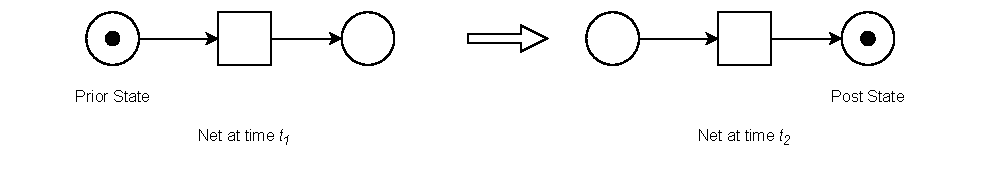
\includegraphics[width=\textwidth]{graphics/PN_Transduction.pdf}
\caption{\textbf{Transduction:
}The transducer is represented as a square node, which will fire when a condition of at least one token as input place value is satisfied, giving rise to the resulting place value.
Places are represented as circles with or without tokens (the values).}
\label{transduction}
\end{figure}


However, a pull action from the complement muscle between the cycle can generate a halting action in between.  Thus two actors can regulate each other's action without involving any other controlling agent or actor. A fine-grain halting may lead to greater coordination.  This is one model of implementing a simple haltable-action-pattern (HAP). 

Haltability, coordination of actions, emerges due to dynamic antagonism among the zones. Having established the fundamental principles of action and haltability, we now turn to the specific biological architecture that implements these principles. The SMN model proposes that cognition emerges from a particular body plan that is shared across animal life but has been largely ignored in cognitive science.

\subsection{Evolutionary Biology of Anatomical Disengagement}
\label{subsec:evolutionary_disengagement}

The capacity for haltability that underlies cognition has deep evolutionary roots. We can trace the emergence of cognitive capabilities through what we call the \textit{evolutionary biology of anatomical disengagement}—the progressive decoupling of body functions that enabled increasingly sophisticated action patterns.

\subsubsection{From Harder-Actions to Softer-Actions}
Let us call the tightly-coupled actions as \textit{harder-actions} (e.g. the coupling between locomotion and feeding in the earthworms), and the decoupled actions as \textit{softer-actions}. During the course of evolution more anatomical disengagements may have given rise to the availability of more such softer-actions.

These examples indicate how one could speculatively weave a story of the evolution as a story of decoupling the body into multiple zones, where each zone can act partially independent from another, and exhibit a distinguishable action pattern. The development of tongue, lips, jaws, pharynx, larynx, gills, lungs, fins, tails, ears, eyes, limbs, toes, fingers, neck, shoulder, hip and so on are interpreted in this story as anatomical disengagement (or decoupling). One can draw a tree of anatomical disengagement representing the epi-physiological bifurcation over and above the phylogenetic tree of evolution.

For example, in early vertebrates as in cephalopods, the feeding and breathing action patterns (filter feeding habit) are not decoupled. In Gnathostoms, we see the stoma (mouth) differentiated through the evolution of jaws enabling decoupled breathing habits from feeding habits. Episodes of decoupling could be reconstructed for the evolution of simpler buccal cavity differentiated into complex cavity, developing teeth, tongue, lips, pharynx, larynx etc. In parallel, an undulating body (as in lampreys) gets decoupled into localised and bilaterally symmetrical fins, decoupling locomotion as a entire-body function. Similarly, one could consider the decoupling of the undulating alimentary canal from the entire undulation of the body.

These episodes of differentiation might have been naturally selected because of the economic value of decoupling, as localised movement is inexpensive than whole body movement. Each episode of such differentiation is an episode of decoupling leading to the evolution of independent action patterns (habits). Thus the gradual polarisation and bilateral symmetry of the body-plan through evolution leading to differentiation of action zones can be woven into a phylogenetic story of decoupled and localised zones of action patterns (habits).

\subsubsection{Economic Dimensions of Disengagement}
This disengagement has an economic dimension, without which it is difficult to understand how it could have played a role in natural selection. The agent can do more work with less effort (spending less energy) because of disengagement. A body plan of an organism that has a coupled movement for both ingestion and locomotion is expensive, than when they are decoupled. Moving when not eating, or eating when not moving is a new found possibility.

Once we have multiple softer-action zones, it is possible to rest some while the others are active. This is the context for the genesis of \textit{haltability}. Haltable variations, one can speculate, could be sexually/culturally selected. The principle of economy also enabled the organism to perform one action while halting another. Isn't this how we describe modulation? The aspect of control we ascribe to modulation arises only when we hold one variable while modifying another. Can we use this insight to ground the regulatory actions required for cognitive processing in haltable action patterns? We demonstrate how this can be the butterfly effect in cognition.

\subsection{The Principle of Layering}
\label{subsec:principle_layering}

Since modulating certain beats such as heartbeats is not affordable, we may consider situating actions over and above the core physiological mechanisms. In order for the actions to be affordable, the interactions of the sustaining layer must continue, and they should generate sufficient surplus. When we say cognition is enactive, it implies that the emancipation from sustaining mechanisms is expensive. Though autopoietic mechanisms may include actions, they are uninterruptible, hence no liberty to introduce gaps here. Hence autopoiesis as a mechanism to compensate the lost energy and matter takes care of the sustaining layer and provides the necessary surplus in the system making actions possible \cite{maturana1991autopoiesis}. This is also an action, but the uninterrupted pace at which this action takes place has no liberty for introducing \textit{gaps} in this layer. In other words, the system can't physiologically afford to halt. However, it is this state that could enable ephemeral actions on the periphery of an autopoietic system whenever and wherever possible. This is made possible by a differentiated body plan that enables a division of labour. Some layers are busy in not only replenishing the loss of energy and matter but also generating surplus energy and matter, such that other layers in the body can \textit{halt}. This design now has room for free action. In this perspective, it is an uninterrupted action of some layer that grants freedom to some other layers. It is this partial break from uninterrupted work, that gives rise to the freedom to enter into the cognitive domain. It is in this subtle sense, that our model differs from Maturana and Varela's account of the connections between biology and cognition. The subtlety we introduce is haltability.

This differentiation of layers, as against the uniform distribution of work, in a system facilitating deviation from the normal course of actions, gave rise to the roots of cognitive state. We shall call this \textit{the principle of layering}, which is over and above the design principles of polarization and asymmetry we discussed earlier. The sense of being over and above can be characterised by naming metaphorically, this principle as epi-physiological or epi-biological.

\subsection{Cognitive Space as Memetat: The Geometric Semiotic Habitat}
\label{subsec:memetat}

Building on the principle of layering, we now introduce the concept of \textit{memetat}—the cognitive space that emerges from the SMN architecture. Cognitive space is a transient geometrical space, \textit{memetat}, constructed through multiple, recursive, recurrent, and haltable serial action patterns, called \textit{memets}, which can be retained by reenacting and creating interpretable traces. The agent's body is modeled as a layered sensation-modulating network (SMN), which is functionally distinguished into a differentiating and filtering network (DFN) and an integrating network (IN).

The SMN is modeled as a polarized and bilaterally symmetrical PetriNet (PN), a bipartite graph of transitions and places. A set of place nodes of the PN enter SMN from the environment where the cognitive agent is situated via the interfacing nodes of transitions. The transition nodes of the PN are sensory transducers and actuators, constituting the sensory-motor part of the architecture. The resulting tokens from the sensory-motor part of the network form as the other set of the place nodes of the PN in the form of a nested stack of neural connections holding transient tokens for a while. The tokens pass through one stack of network into another until they vanish completely. The phenomenological space is constructed by the tokens in this transient nested stack of networks through multiple, recursive, recurrent and haltable serial action patterns by the sensation-modulating network.

The geometry is computed by calculating (1) the differentiation of differences in the phenomena through self-modulation, (2) the relative location of the phenomena following the principle of \textit{mapping the delay with distance}, and (3) the principle of the concomitance of phenomena granted by a dynamic \textit{fire-together-wire-together} architecture of the SMN. The spectrum of perception to conception (spectrum of abstraction) is explained through a model of a spectrum of saturation of multiple sensory modalities and the corresponding dynamic spectrum of engagement and disengagement of action patterns. Meaning and evaluation are grounded in the deeper layers of the layered architecture of the SMN. Transient action patterns can be memorized and recalled only by re-enacting them, while the traces of action patterns can be persistent and hence can be recalled and gamified. Human culture is modeled as a confluence of multiple microworlds, where each microworld is constructed by mutually stimulating rules following actions that define the boundaries of the transactional playground.

\subsection{Biological Architecture for Cognition: Tubular, Polarised, Nested, Serial and Bilaterally Symmetrical Body Plan}

The broad body plan of a cognitive agent is tubular and topologically a torus. Most multi-cellular organisms during development indicate that the underlying form is that of a torus. Specialized morphogenesis, leading to differentiation, results in the final shape appearing differently, but the fundamental toroidal structure remains.

The 3 components of concern for a cognitive architecture are (1) the sensory receptors organised as \textit{sensory boards (SB)}, (2) the motor action zones organised as \textit{motor boards (MB)} and (3) the connectors in between sensory and motor boards organised as a \textit{network}. Thus the body of a cognitive agent is modelled as a sensation modulating network (SMN). The nodes of the network include sensory and motor boards, while the edges include the connections of the network. Biologically, sensory boards are realised by sensory receptors, motor boards by the muscular and skeletal system and the edges of the network (connections) by the nervous system.

It is important to keep in mind the contrasting point of the architecture with the received view that confines network only to the nervous systems, where the body of the neuron, the soma, forms the node, and the axons and dendrites form the connections. In our model, the entire cognitive agent's body is a network, with the nervous system providing only the differential connections between different sensory-motor subsystems. 

Sensory receptors are located in a distributed way across the body in the outer, inner and middle layers. The distribution of these nodes \textit{on} and \textit{in} the body is not uniform. Polarization exists, in the sense that some nodes are arranged densely on one-side of the tube. For example, a pair of eyes are located towards one pole of the body and absent at other places. Each eye has multiple photo-receptors and motor modulators, together constituting the nodes of the network. Similarly we see such concentrations of sensory receptors for other modalities. Although tactile receptors are located in a distributed way, their density varies from place to place on and in the body. This unequal distribution in location and density of sensory receptors plays an important role in differentiation and solving the problem of location.

The sensory receptors are differentiated into specialised modalities transducing thermal, tactile, auditory, visual, olfactory, gustatory and location signals. The polarised and bilaterally symmetrical arrangement of these sensory receptors plays a significant role in constructing the picture of the internal and external world. The receptors organised as sensory boards are \textit{mounted} on the motor and mechanical boards (muscular and skeletal system). One more contrasting point of this model may be noted, that we consider the motor boards as sensory receptors of location, and not merely as actuators. As far as cognition is concerned, actuation is essentially for supporting sensation of every modality, committing to the theory of action based perception. 

On this body plan, there are also multiple action zones. It is important to note that action zones are also oriented towards the inner layers of the tubular body plan of the agent. There are more action zones at the anterior side, particularly at the inner surface of the tube, making the body polarized. Animal anatomy describes this plan often in the name of cephalization \cite{hyman1940invertebrates}, seen in almost all bilaterally symmetric beings. 

Apart from the polarised distribution of sensory organs, it is important to note that the motor organs, which are also sense organs, are located in a \textit{nested} manner across the body.

A large set of highly specialized motor receptors (location sensors), are present across the body organized in a bilaterally symmetrical and hierarchical (nested) manner, which biologists call as skeletal or voluntary muscles. In our model, insofar as cognition is concerned, skeletal muscles are sense organs, and their movement directly supports perception. Biologically, muscles are considered as organs of movement and locomotion. In conventional cognitive science, their role is considered auxiliary. In our model, movement and locomotion are primarily cognitive functions. Apart from providing location data as a sensory subsystem, their \textit{characteristic} movement provides conceptual schemes employed in cognition.

The motor receptors of the network are unique, because they are mounted/embedded in a bundle of muscle fibres organised as \textit{boards}. This specialized plan is essential for playing the role of \textit{inferring} the location. The data from location sensors is created through movement. That is to say, the position is resolved only by change-in-position (displacement). But, location cannot be determined without data from the other sensory streams. We interpret location, like consciousness, as a dispositional concept. Location is always of some thing or the other, some sensation or the other, of some phenomena or the other. Employing a Kantian aphorism, we may say: location without sensory data is empty, and sensory data without location is blind. Moreover, it is not only that location cannot be calculated without movement, the construction of an image of the world through other senses is impossible without spatio-temporal data. Action is essential for resolving both space and time.  

The source of temporal data is the serial action pattern.The body plan is not only polarised and nested, but also serial in nature. We also assume availability of repeatable actions, beats within the body, providing a temporal canvas/ stage. The availability of the temporal stage/ canvas is granted by the existence of metabolic cycles, biological clocks is well established [cite] in terms of diurnal and biurnal rhythms.

Antagonistic action is a key character of the body plan, which plays an important role in the current model. 

The body is not a complete network. The model uses the principle: ``Fire together. Wire together'' (FTWT) \cite{hebb1949organisation}. The SMNs that are recurrently active at the same time are likely to get connected over a period of time. Thus the connection `board' is plastic, not static. The connection patterns are created, reinforced and modified based on the dynamics of the body (action patterns) in its ontogeny (developmental history). The implication of the FTWT principle is that the actions determine the connections, and not the other way around. However, much of the differential connections may have been already determined by phylogenetic and prenatal action history. Though it appears as though the agent starts with an undifferentiated state, the phylogenetic and prenatal action history bestows, practically, a body with `innate' action schemas at birth.

In a model where actions are located at the interface between the body and the environment, the actions within the body (including the prenatal stage) are often ignored (e.g. suckling, swallowing action-patterns etc.). In our model, the most stable and determining action schemas are already in place by the time the agent is exposed to the external environment after birth. 

\begin{figure}[ht] 
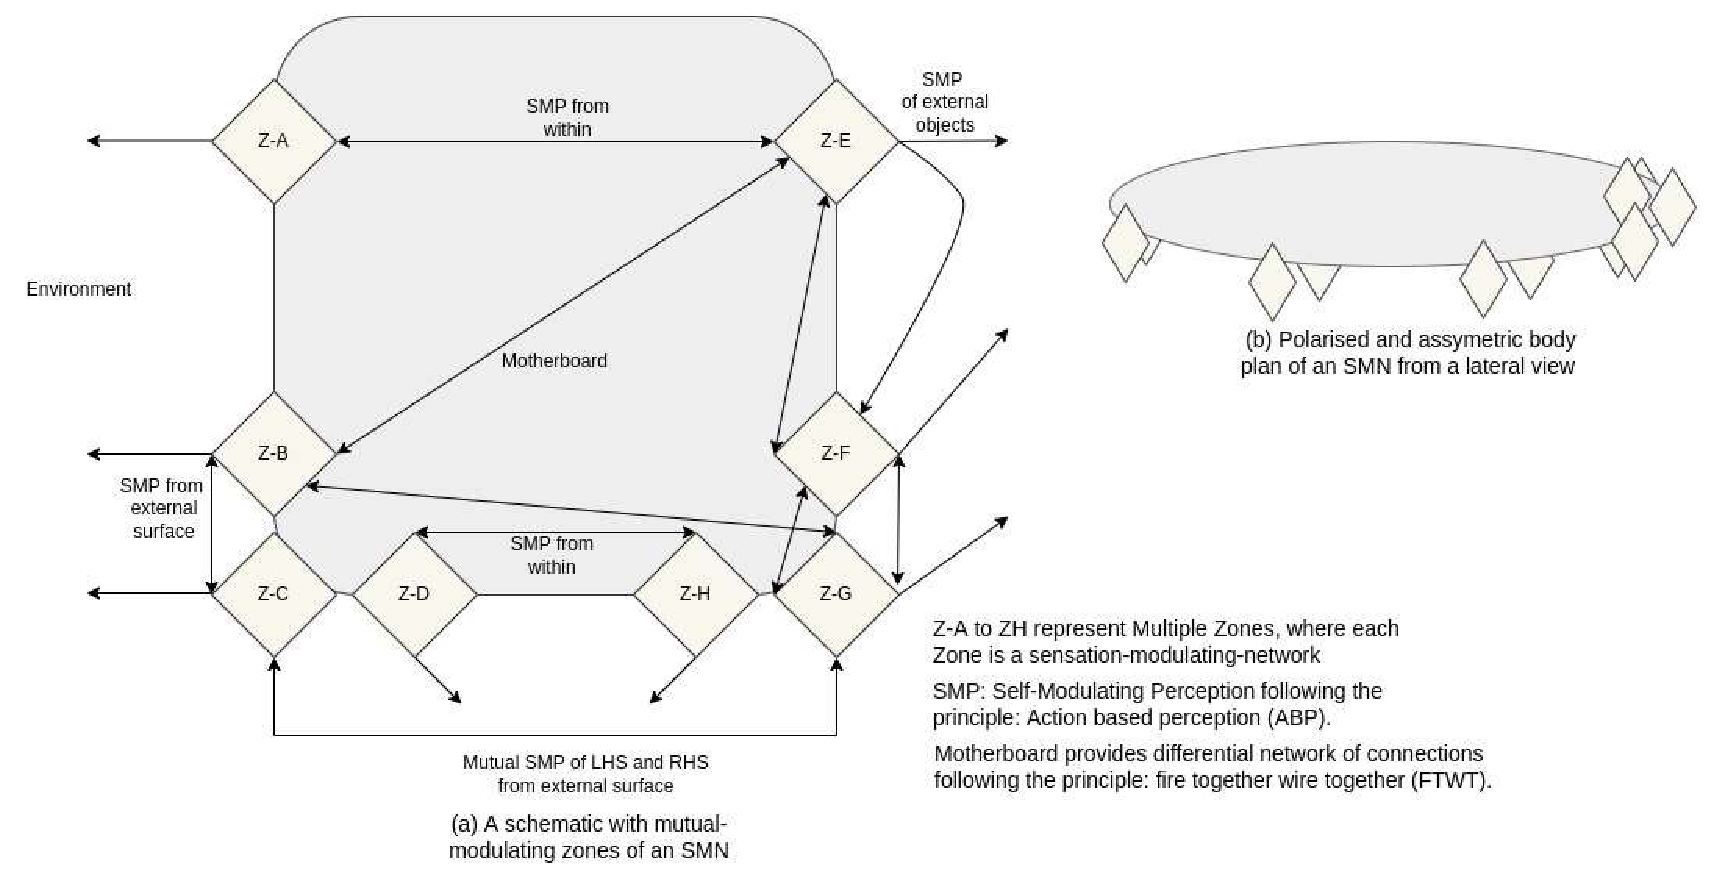
\includegraphics[width=\textwidth]{graphics/self-modulating-perception.pdf}
\caption{\textbf{A schematic representing a cognitive agent as a network of multiple self-modulatable zones.}}
\label{smn}
\end{figure}

Mutual modulation of action within the body is an important and contrasting feature of the model, which is largely ignored in the current discussions in cognitive science. This mutual modulation, within the body, is a core cognitive mechanism in the current model, which appears very early on during the prenatal stage itself. Therefore, we locate the roots of cognition within mutual modulation within the body (internal environment).

The outgoing arrows from the zones represent the sensory modulation from an external world invoking action based perception (ABP) \cite{noe_action_2004}. According to this principle, the perception is not a passive sensing of the world out there, but an active process. The same principle is employed when an action zone modulates another action zone within the body. This implies that ABP is used for perceiving both the worlds (internal and external). The double headed arrows in the figure represent mutually modulating zones. Between Z-B and Z-C, the double-headed arrow represents mutual modulation from the outer surface. For example, consider a fidgeting action between fingers touching side-ways, the hand touching the chin in the typical thinking posture, scratching an itch on the same side of the body etc. The double-headed arrow between Z-C and Z-G represents another mutual modulation from an outer surface (e.g. clapping with hands), LHS and RHS mutually modulating.

In a well-connected body, the implementation of a single-headed arrow between two zones (like Z-E and Z-F) appears very rare. However, to understand such a possibility, we can consider touching a numb leg, where due to temporary lack of internal feedback, mutual modulation is transiently unavailable. The double-headed arrow between Z-D and Z-H could represent mutual modulation between the action zones from within the body. For example, swallowing zone and speech zone. In the case of swallowing, with or without food, the upper and lower surfaces of the buccal cavity, pharyngeal zones mutually touch and modulate each other.

Often, self modulating actions, such as thinking, are considered as recent evolutionary features, whereas in our model, the very root of cognition is due to such internal mutual modulation, though it is counter-intuitive. The world within the body is missed in the current accounts. Since this is a contrasting feature, more elaboration on this follows in the model. 

\begin{figure}[ht] 
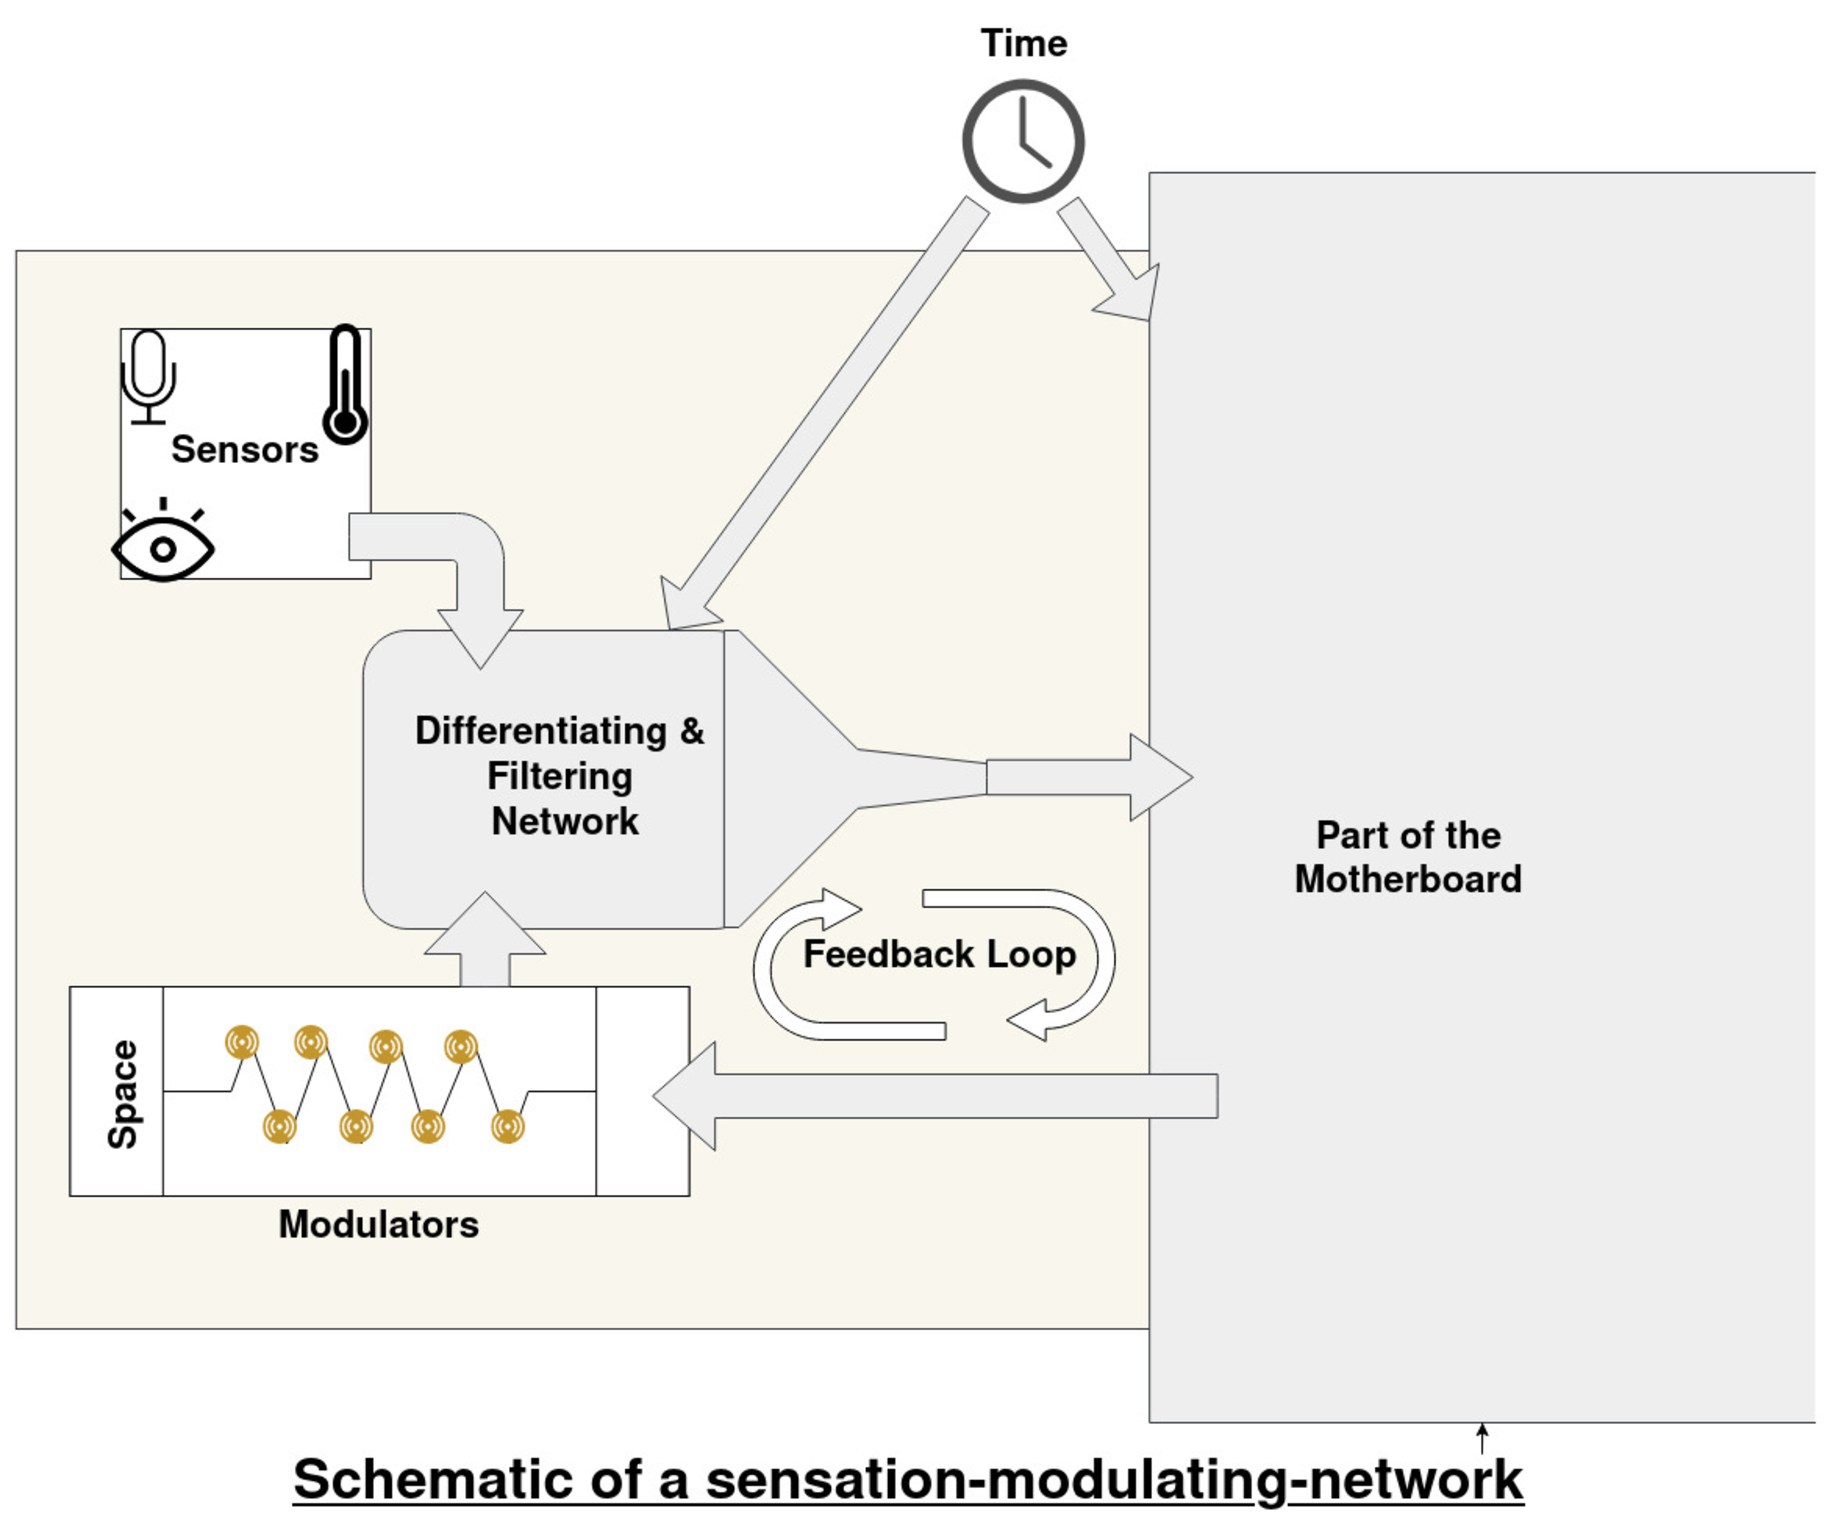
\includegraphics[width=\textwidth]{graphics/structure-of-Zone.pdf}
\caption{\textbf{A schematic of a perception modulating action zone.}}
\label{zone}
\end{figure}

\subsection{A Network of Sensation modulating networks}

The structure of a cognitive agent's body is modeled as a nested network of Sensation Modulating Networks $\{n(SMN)\}$. And the dynamics of cognition is modeled as differentiation of Differences $\{\delta(D)\}$ in a  multi-modal sensory stream.

It is important to underline, as a point of contrast, that the Central Nervous System (CNS) is not interpreted as \textit{the} network in our model, but a part of it. The entire cognitive agent's body is a network. CNS provides only the differential connections between different DFNs and among the nodes (sensory and motor receptors). Therefore the popular schema of brain-body-world is reduced to body-world. Since the body is a network of SMN, this schema can be represented as 
\begin{equation}
[\{n(SMN)\} \rightleftharpoons \{W_I\}] \rightleftharpoons \{W_E\},
\end{equation}

where $W_I$ is the internal world and $W_E$ is the external world.  $W_I$ can be substituted with another $\{n(SMN)\}$, since it is nothing but another $W_I$ in effect. 

Thus the above representation can be re-written as 
\begin{equation}
[\{n(SMN)\}_i \rightleftharpoons \{n(SMN)\}_j] \rightleftharpoons \{W_E\}.
\end{equation}
What constitutes the internal world will become clear once we make the principle of mutual modulation clear below.

This schema can be contrasted with the brain-body-world schema, which can be represented as 

\begin{equation}
\{CNS\} \rightleftharpoons \{B\} \rightleftharpoons \{W_E\}
\end{equation}

where the CNS is the central nervous system, B is the rest of body and $W_E$ is the external world.

Consider the functional network as a $\Delta$ network of a set of sensory boards $\{S_i\}$ and motor boards $\{M_j\}$. We represent this network as 
\begin{equation}\label{delta_notation}\Delta^{\{S_i\}}_{\{M_j\}}, or simply, as  \Delta^{\{i\}}_{\{j\}},
\end{equation} 
where the subscripts always refer to motor boards, and superscripts to the sensory boards. For example, if $S_1$, $S_2$, $S_4$ and $M_1$, $M_5$, constitute a transient network at any given time $t_1$, this state of the SMN can be represented as 
\begin{equation}\label{delta_eg}SMN(t_1) = \Delta^{1,2,4}_{1,5}
\end{equation} 
This $\Delta$ network is an ephemeral functional state corresponding to a particular action performed by the cognitive agent at $t_1$. Thus differentiation of Differences is realised in $\Delta$ networks, where the motor boards differentiate on the Differences streaming from the multi-modal sensory boards. This is how we resolve every action as a functional network of sensory motor subsystems.

Differences are given and taken from the environment directly, while differentiation is an active function of the agent. This active function can resolve modalities and selectively attend to a difference in the stream.

SMNs are functional states of the cognitive agent. This identifiable functional state does differentiation and filtering. Since each SMN is a network, the body is a network of networks. We may represent the active cognitive agent as $\{n(SMN)\}$. The first order network of SMN is a functional sub-graph. By functional subgraph, we mean, it is not distinguished based on structure, but by ephemeral or transient connections. SMN is hence localizable, but ephemerally.

Each sensory board is an array of localised sensory receptors (transducers), which connect through a bundle of connectors (a bus) to a differentiating and filtering network (DFN). Each motor board is an array of location-receptors mounted on a bundle of actuators (muscle-fibers). The motor board connects through a bundle of connectors to the DFN on the one hand, and receives connections from the integrating network (IN) on the other. The DFN and IN are distinguishable only on the basis of their function and the nature of connections, and need not be localized in any specific area of the central nervous system (CNS).

The motor board can be considered as a mediating board between a DFN and IN. In other words, the motor board is sandwiched between the DFN and IN, creating dynamic and transient loops. Speaking of the network in graph-theoretic terms, we can say that, the nodes of an SMN are arrays of receptors and actuators, and the edges are dynamically distributed bundles of connections manifesting the aforementioned loop.

\begin{equation}
[\{n(SMN)\}_i \rightleftharpoons \{n(SMN)\}_j] \rightleftharpoons \{W_E\}.
\end{equation}
What constitutes the internal world will become clear once we make the principle of mutual modulation clear below.


This schema can be contrasted with the brain-body-world schema, which can be represented as 

\begin{equation}
\{CNS\} \rightleftharpoons \{B\} \rightleftharpoons \{W_E\}
\end{equation}

where the CNS is the central nervous system, B is the rest of body and $W_E$ is the external world.


\subsection{The Functional Model of the Cognitive Agent}


In this section we present an argument that the human cognitive life, for that matter of any other cognitive agent, cannot be explained without an asymmetrical ontology and a gap-creating epistemology.  

\emph{The asymmetry condition is satisfied by polarized body plan and a bilaterally symmetrical localization of sensory and motor boards.} The asymmetry condition is satisfied by polarized body plan and a bilaterally symmetrical localization of sensory and motor boards. 
The structural body plan provides an embodied action schema for grasping the world. It is more natural for most of the animals to walk, run, swim or fly forward than backward because of the body plan. The architecture of the limbs of all the terrestrial organisms is asymmetrical, based on a limited degrees of freedom at each joint. Polarized orientation of the body to the ground with ventral and dorsal body differentiated, facilitates dealing with the field of gravitation. 

\emph{A formatted body and its action patterns determines the structure of the phenomena.} Specialized sensory boards are also organized to suit this body plan. As a result, the possible action schemes can resolve the structure of the world. This resolution is logically impossible without movement, and most importantly the patterns of movement facilitated by the body plan. The problems of cognition cannot be resolved without addressing this basal mechanism. Mere sense organs and the nervous system are not sufficient to build a complete framework. The nervous system cannot process the data stream coming from sensory organs without a mediating and modulatory system. Data can be stored only if we have a formatted body. The format of the body is not only the structure, but also the format of actions. The action patterns depend on the body, modeled as a sensory-motor network.  We shall elaborate on how this model could ground cognition in this section.

\emph{Framing problem} A stream of uninterrupted sensations may have a pattern, and it can be processed to identify the pattern. But this is an ungrounded process, because, \textit{on its own} the machine cannot detect: Where does the stream come from, from within the machine or outside? Which pattern to attend to? Which pattern is more significant than the other? Which ones to ignore? This is the framing problem. This problem is related to how a cognitive agent understands the context/situation. 

\emph{Naming problem} Apart from the understanding of context, we need to deal with naming and referencing. Information processing is not only impossible without names but also useless if it cannot name the patterns. One may program the machine to give distinct names to distinct patterns, and can also group them nicely based on some similarity detecting algorithms. But how does the machine establish a reference, of which patterns pertains to which object in the world, or within the machine? And more importantly how could it convey to us the \textit{private} naming convention?  Can the machine at least tell them to itself?  If so how? These are three philosophical problems at one go: concept formation, symbol grounding problem and that of possibility or impossibility of a private language. Variation in the world and a capacity to detect patterns in a stream of experience is not sufficient to give names to the patterns. We need a naming mechanism in a cognitive agent, and we need a mechanism to communicate with each other, in a community of agents, through names. Let's call this \textit{the naming problem.} 

Combining the above two problems, let us call them together a \textit{naming-framing problem}, because we think that the frame problem and symbol grounding problem are intrinsically related. 
We will now argue that the naming-framing problem can be solved through modulation. In other words, referencing and distinguishing the external world from the internal world will be shown to be possible through the same mechanism. 

\marginnote{The principle of layering} Since modulating certain beats such as heartbeats is not affordable, we may consider situating actions over and above the core physiological mechanisms. In order for the actions to be affordable, the interactions of the sustaining layer  must continue, and they should generate sufficient surplus. When we say cognition is enactive, it implies that the emancipation from sustaining mechanisms is expensive. Though autopoietic mechanisms may include actions, they are uninterruptible, hence no liberty to introduce gaps here. Hence autopoiesis as a mechanism to compensate the lost energy and matter takes care of the sustaining layer and provides the necessary surplus in the system making actions possible \cite{maturana1991autopoiesis}. This is also an action, but the uninterrupted pace at which this action takes place has no liberty for introducing \textit{gaps} in this layer. In other words, the system can't physiologically afford to halt. However, it is this state that could enable ephemeral actions on the periphery of an autopoietic system whenever and wherever possible. This is made possible by a differentiated body plan that enables a division of labour. Some layers are busy in not only replenishing the loss of energy and matter but also generating surplus energy and matter, such that other layers in the body can \textit{halt}. This design now has room for free action. In this perspective, it is an uninterrupted action of some layer that grants freedom to some other layers. It is this partial break from uninterrupted work, that gives rise to the freedom to enter into the cognitive domain. It is in this subtle sense, that our model differs from Maturana and Varela's account of the connections between biology and cognition. The subtlety we introduce is haltability. 

\emph{Homologous roots of anatomical disengagement, modulation and haltability} These examples indicate how one could speculatively weave a story of the evolution as a story of decoupling the body into multiple zones, where each zone can act partially independent from another, and exhibit a distinguishable action pattern. The development of tongue, lips, jaws, pharynx, larynx, gills, lungs, fins, tails, ears, eyes, limbs, toes, fingers, neck, shoulder, hip and so on are interpreted in this story as anatomical disengagement (or decoupling). One can draw a tree of anatomical disengagement representing the epi-physiological bifurcation over and above the phylogenetic tree of evolution. 

Lets call the tightly-coupled actions as \textit{harder-actions} (e.g. the coupling between locomotion and feeding in the earthworms), and the decoupled actions as \textit{softer-actions} \cite{nagarjuna_muscularity_2005}. During the course of evolution more anatomical disengagements may have given rise to the availability of more such softer-actions. 

We need to cut the story short to revert back to how the transformation of a tightly coupled body plan into a loosely-coupled body plan, from harder-actions to softer-actions, is relevant as a context for cognitive science. The cognitive hypothesis we propose, given this transformation of the body plan, is: the greater the disengagement of differentiated action zones, the greater is the agent's capacity to modulate the incoming stream of experiences. This disengagement itself is a function of anatomical polarization and layering. 

Once we have multiple softer-action zones, it is possible to rest some while the others are active. This is the context for the genesis of \textit{haltability}. Haltable variations, one can speculate, could be sexually/culturally selected. The principle of economy also enabled the organism to perform one action while halting another. Isn't this how we describe modulation? The aspect of control we ascribe to modulation arises only when we hold one variable while modifying another. Can we use this insight to ground the regulatory actions required for cognitive processing in haltable action patterns?  We demonstrate how this can be the butterfly effect in cognition. We now move to discuss how haltable-action-patterns (HAPS) can become units of analysis for cognitive \textit{behavior}. 

\emph{Homology of FAPs and HAPs} This story has affinities with the view that dexterity and movement of the body contributes substantially to cognition \cite{bernstein2014dexterity}. And in cognitive neuro-science the emphasis has always been on how CNS or brain modulates motor actions. In the context of the current model, it is important to mention the concept of fixed action patterns (FAPs), which are no different from the multiple softer-action zones mentioned above. As Llinas argues the synergistic coordinated action of a cluster of muscles take part in \textit{fixed action patterns} (FAPs), which play an important role in his narrative of how to build mind from body \cite{llinas2002vortex}. In fact the choice of the expression haltable action patterns (HAPs) is inspired from Llinas, which suggests the contrasting feature of our model with that of Llinas. 

What is the role of halting in cognition?
Recalling the structure and dynamics of the SMNs explained in the above section (see figure\{\ref{zone}\}), we presented a view where the incoming stream of sensations go almost unnoticed without modulation. In an architecture where the sense organs are mounted on the available multiple modulators, the stream of sensations change in accordance with the action performed. This correlation binds the sensation with actions giving rise to perception. This is in line with the positions of Merleau Ponty \cite{ponty1969phenomenology} and Alva Noe \cite{noe_action_2004}, who argued for an embodied and enactive view of perception and cognition. 

In the synergistic motor assembly of FAPs, which is essentially a sensori-motor assembly, the foundations for modulating sensation may have been laid providing a mechanism for DFN. 

The fundamental question that we can ask is: What makes modulation possible? In the current views in cognitive sciences, modulation is typically managed by the brain; therefore researchers seek to locate the zones/ regions of control within the brain. By contrast, in our model, by suggesting that there is a strong link between haltability and modulation, we locate the mechanism in the zones of disengagement. In this interpretation, the anatomical disengagement, the ability to halt, and the ability to control are homologous. The terms used to describe higher order cognition --- `modulation', `regulation' and `control' --- are gross descriptions of phenomena, whereas haltability rooted in anatomical disengagement is a more nuanced and observable description of the phenomenon. Further, it avoids the need to identify a part or the system as an organ of control, instead ascribes this to the entire SMN, as a systemic ability. Therefore resolving modulation in terms of haltability adds greater rigor by providing an observable criterion for modulation. 

\emph{Rooting Epistemology in the gaps} As detailed above, the disengaged motor assemblies are capable of acting independent of others. The effective capacity emerging out of this is the potential to remain transiently inactive. The pattern of halting provides the structure for the rest of the story. 

\emph{Rooting syntax in a sequence of HAPs} As we understand from the theories of information, the logical conditions required for variations can be provided by gaps. For example, in a minimalist possible code, such as Morse code, the patterns of dots are created with interruptions (gaps). The various possible patterns of truth and falsity or 0 and 1, used as a foundation of encoding and processing in computer science, demonstrates the potential of gaps in generating variations. Introduction of \textit{gaps} makes syntax possible, which in turn enables the generation of as many patterns as required. Since the practical needs are a small subset of the logically infinite number of possible patterns, this is sufficient for encoding knowledge. In sequential patterns, syntax and pattern are identical i.e., they are two sides of the same coin. Syntax is a feature of sequential patterns, which can be grounded in the patterns of halting. 

\emph{Arbitrary mapping} However, understanding how to generate numerous action-patterns is apparently a simpler issue than decoding the action-patterns and their reference (what they stand for). Because, action-patterns can be generated arbitrarily as well. It is also possible to map any arbitrary action-pattern to an arbitrary reference. However, in a given context, the mapping is required to be \textit{conserved} for semantic coherence over time. This fixing the map between an action-pattern and what it could stand for does not make sense without reproducibility and continued conservation of the mapping of the action-pattern to the reference. 

\emph{Memories are reproducible action-patterns} Reproduction of an action-pattern is possible without binding it to a reference. For example, a melody generated either by an instrument or orally, does not have to stand for any reference, or they could stand for multiple references, making them ambiguous. It is a feature of artistic creations to escape from a stable reference. A general feature of melodies is that it is hard to forget. Given the fact that melodies are generated by action-patterns, we could consider what we remember are like melodies. We agree with the view that memory is \textit{for} action\cite{glenberg1997memory}, but we also argue, as a framework based on action ontology, that reproducible action-patterns and/or their traces \textit{are} memories. 

Enacting an action-pattern and decoding what it stands for can be distinguished. 
The capacity to decode an action pattern requires holding on or recollecting the mapping with a reference. 
The entry of reference in our discussion is necessitated by a separation between an object and its \textit{name}.
Let's use the example of talking about a cup by hand-grasping-a-cup action-pattern (gesture). 
\emph{Entry into Semiotic world} The possibility of grasping action-pattern \textit{without an object} (in this example, a cup) is a significant bifurcation point and an entry into semiotic world. 
The miming action of grasping an object can become a \textit{name} for objects. 

The mime for holding a pen, brush, liquid, cup, basket etc. could all be different, based on the affordances these objects offer to the agent. Grasping any object is saturated, while a mime of grasping without the object is unsaturated. 
Mimes can stand for not only objects but also verbs. For example, we can sign someone ``to get in'' or ``to get out'', as well as ``please come in'' or ``you may go now''

If the action patterns are always \textit{saturated} with the object or event, they can never become names for them. Naming is impossible without breaking this contingent binding. We therefore consider unsaturated action-patterns as a necessary condition for a semiotic life, where naming action-patterns are separated from the object they stand for. 

An action-pattern could be bound to a reference in a \textit{hard} or \textit{soft} manner. Harder binding specifically applies largely to gestures (inter-subjectively presented action-patterns). 
The action-pattern used as a mime, when closely related to the affordances offered by the object or event, are harder. 
Some mimes transcend the affordances of the object or an event, since they hold no morphological or functional correspondence to them. \emph{Possible relation to modal and amodal concepts} For example, in a typical Indian classroom, when a student stands-up in the middle of the class and shows his/her little finger, the teacher as well as the rest of the class understand that the student is seeking permission for a bio-break. This may not work in another culture. Because the binding between the little-finger-mime and seeking permission for a bio-break is created \textit{arbitrarily} without any match with the affordances. Whereas using a thumbs up mime to seek permission or a hydration-break is less arbitratry and matches with the affordance of drinking water. 

While the possibility of hard-mimes could be a major bifurcation point for communicating agents, the use of soft-mimes for communication is a revolutionary bifurcation point, because this breaks open a world of possibilities. 
We think that this could be the episode of punctuated equilibrium\cite{gould1977punctuated} in the evolution of homonids. The communities that could use arbitrary mimes (names) had a political and economic advantage over other communities, because arbitrary names gives rise to proprietary/ private (closed group) languages.\cite{corballis2014recursive}

Once we move from gestures as mimes to the traces of action-patterns, such as the sounds or inscriptions standing for an object or event, the separation between them is so deep that it is difficult to decode them by simple correlations without training or lived experiences. 
Affordances of objects and events, in the world of traces of action-patterns, hardly help to decode. Some traces of action-patterns, such as inscriptions that bear a similar morphology to an object or an action, e.g., smilies, are harder (closer to the reference). But enter the world of alphabets used to create names we enter into the ``software'' world of representations. 

Enter the ``software'' world, we enter the world of rule following games. Thus the mapping between the patterns and their references provides the rules. 
This jump from action-patterns to rules is not a step taken but a major leap. 
Rule following action-patterns provide a spring-board to another world. 
So, we need to halt by asking the question: what makes rule following games possible? 
This is a highly involved problem, since we have suddenly entered into a context of a community of agents, and not merely an individual agent. 
This cannot be resolved unless we demonstrate how in the proposed model, we can account for shared memory and shared experiences in a community of agents. 
We shall indicate an approach of resolving this problem, if not actually entirely solving, here. 

\subsection{Co-construction of memetat and self-identity}

\emph{Recurrent self-modulated action-patterns become habits. Every habit has an inherent syntax. These HAPs are \textit{action schemes}\cite{piaget1970genetic}.}

One of the first outcomes that an SMN needs to make in the model presented above is to differentiate the experiences into what is in the body and what is outside the body. 
The modulations of perceptions of one zone affecting the other zone happen at the same time, and therefore these zones get connected through FTWT principle. 
There exists a reinforcing loop, because of the fact that the two zones obtain stimulation at the same time. For example, thumb/toe sucking action observed in the fetus prior to birth, has simultaneous stimulation from two zones viz., the thumb/toe zone and the buccal zone. 
On the other hand, the fetus kicking action-pattern on the walls of the womb of a mother, are those action patterns where one SMN is stimulating another SMN. These are two independent networks. 
Though the stimulation happens at the same time, the reinforcing loops within the network do not exist. 

After birth when a child kicks the crib, an SMN is acting on a non-SMN. This action does not have a reinforcing loop in the SMN. So the crib is outside the body. So are the rattles and teddy bears in the vicinity of the child. 
As far as the active SMN is concerned the boundary between the body and the world is clearly drawn. No scope of solipsism here. The phenomenology of objects within the internal network and the external world are different. 

An embrace between two bodies (SMNs), say between a mother and a baby, is another case. Here two networks are mutually self-stimulating by both the SMNs enacting similar HAPs. Multiple zones are stimulated on each body at the same time, resulting in an inter-subjective feedback that reinforces the synchronous synergistic bonding. Here, even though the SMNs do not have direct connections at the network level, they are connected by synergy developed through synchronous self-stimulation and their effects. Such HAPs are repeated for the mutual positive reinforcement leading to conservation of an inter-subjective space. This is absent when a child kicks the crib. When the fetus is kicking the womb, it may appear as if two networks are acting on each other, but the only actor there is the fetus, for the mother's womb has no self-modulating capacity. Therefore, mother's body is practically an external environment to the fetus. In the above 3 cases, we have 3 different situations of the modulation --- in the crib kicking case, the baby modulates and experiences, but the crib does not; in the womb-kicking case, the fetus modulates and experiences, but the mother is only at the receiving end; whereas in the case of embrace, SMNs of both the baby and the mother mutually modulate and experience, and hence we can ascribe an inter-subjective space here.  In such an inter-subjective space the agents are not merely acting, but \textit{transacting}. This transition from action space to transaction space is the entry into \textit{memetat}. 

An infant kicking a rattle is yet another case. The generation of sound at the time of kicking the rattle is an example of self-production of sound. This also generates interest (attentional anchor), since this is in effect a zone (kicking zone) stimulating other zones (hearing zone, touching zone, visual zone etc). This exploration is motivating due to one's ability to control the production of changes in multiple sensory modalities. Similar example is when the child kicks a ball: when they kick the ball, though the ball is not part of the network, the other zones --- audio-visual-haptic zones --- provide the temporally correlated events. This action when repeated binds the experiences resulting from action. This is also a loop nevertheless. But the internal feedback loop is absent. Correlation is not a sufficient indication of causation, similarly firing together is not a sufficient indication of causal connection. In the thumb-toe sucking case on the other hand, the loop gets closed with a greater degree of certainty. Even in the case of kicking a rattle or playing drums, though there is no direct closure of the loop, there exists experiential closure leading to incorporation of the object into the agent's action-experience space. Often we enter into this recreational zone when we dissolve into a \textit{flow} \cite{Mihaly}. 

When a child holds a bat and explores the world outside though the bat is not part of the network, it provides haptic experiences extending the SMN's action space becoming part of its peri-personal space. 

The possibility of holding zones such as hands, beak, mouth, etc. is yet another major bifurcation point. The external object that the agent can hold extends the explorations and experiences, beyond what was affordable through the body itself. For example, objects that are hotter or sharper or heavier etc. can also become part of the explorable and experientiable spaces. Thus, a combination of tools with holding action zones, extends the action space leading to extended the habitat as well as perceptual space. 

The action patterns as mentioned above, become habits, and the habits become names (initially as gestures) the corresponding external objects become part of the habitat (explorable and experientiable spaces) which turn into memetat (transactable spaces). 

One may take several such examples to understand how the SMN can demarcate internal world from external world. This abstraction of internal and external is operational, and participates at the root of constructing \textit{self} and concept formation at the same time. Interestingly, the formation of self is not independent of the formation of what is not self. The context of operations/actions that are germane to the separation of the internal and external and the context of operations that are germane to the separation of the self and the-other (non-self) are not different. They are co-constructed, as a thematic pair. This is how a sensation modulating network or sensory motor network as an SMN acquires an entry into a cognitive ground. 

\subsection{Nested HAPs}

Having alluded to the possibility of naming through haltable-action-patterns, and the memet-memetat differentiation, we shall now address how nested-action-patterns can be constructed through self-modulation in an SMN with multiple zones of HAPs. 

\emph{Representing the complexity of nested HAPs} Clapping can be done, while the body is standing, sitting, walking, talking or running etc. The clapping action zone is disengaged from the other states the body could be in, i.e., it could be performed independent of the rest of the states. The nesting of action patterns can be represented as [sitting(clapping)],  [talking(clapping)],  [running(clapping)],  [walking(clapping)],  [singing(clapping)] etc. The nesting becomes complex when we keep walking, while singing and clapping [walking, (clapping (singing))]. The variations in nesting can be seen when the frequency of walking and clapping match, or some modified patterns through skip-clapping, while singing action pattern is going on. 

\emph{Iterative, recursive and alternative sequences of HAPs} In order to generate a sequence of HAPs performed at different zones, it is necessary for the zones to have the capacity to act independently. We shall use the term `iterating sequence' referring to repeated actions in the same zone. We shall use `recursive sequence' when actions involve multiple zones, and when actions can happen together. In the case of alternating action patterns involving multiple zones there is no recursion. We shall use the term `alternating sequence' for this case. Thus there can be 3 types of sequences that are distinguished:  iterative sequence, recursive sequence and alternating sequence. Recursive and alternating sequences can also be iterated. These form the syntactical aspects of HAPs. The core logical requirements of richer syntactical representation are satisfied by HAPs that can be iterative, recursive and alternative. 

Though, iteration implies a sequence of repeated actions, distinguishing an iterating sequence and a recursive sequence is significant for understanding semiotics. Alternating the iterative and recursive action patterns is the basis for the creation of rich symbolic forms. Logically, HAPs are required for creating such variations. It may appear logically sufficient to create variations in a sequence involving a single zone to generate syntax, e.g. Morse code.  However, it is cognitively insufficient, because the gaps can not be recognised without a reference clock (another iterating action sequence). 

The zones that are in a state of recursive HAPs, which are synchronous, can be considered as the roots of the nested structure. For example, a person clapping a simple rhythmic beat while tapping the feet alternately, left-right, is a very simple nested structure. Here the alternating-tapping is nested in the clap-beat. One can increase the complexity by arbitrarily moving another zone such as turning the neck left to right while also doing the alternating-tapping. The alternating-tapping and the alternate-neck-turning are nested inside the clap-beat. It is up to the creativity of the choreographer, to play with the endless possibilities of modulating haltable zones within the bounds of the body architecture. 

Let us take another example of clapping while walking forward, backward, sideways while also turning the neck, hips, shoulders etc. All these actions may happen in a sequence or may happen while holding one zone in a fixed or a stable recursive action-state as a beat. The beats need not be performed from within one body. When more than one agent is participating, then the sequences and the beats can be performed either sequentially or synchronously. The permutations and combinations of these possibilities are endless, even in this simple example. When the speech zone enters, then we add to the complexity, further. 

However, the number of such zones that are available for creating alternating nested sequence, in a context, determines how complex the symbolic life of that agent can be. Can't this be one of the comparative parameter of cognition among agents, both within and across species? These abilities can not be taken for granted in a body architecture, for they may not be realised without situating in suitable social and natural contexts. 

\emph{Creating and recreating internal world} Considering the speech as a peculiar ability of human-body, it is important to understand that it is not a single zone of action, but involves multiple zones. Apart from employing multiple zones in speech, all the actions are self-stimulating/ self-modulating as well. For example, the left and right and the top and bottom parts of the complex vocal apparatus touch each other: lips, tongue, pharynx, larynx stimulate each other in a variable sequence while modulating the inhalation and exhalation halting patterns. This is a paradigm example of generating a complex sequence of self-stimulating perceptions, because the body is not acting on an external object, but on itself. This introduces a complex phenomenology that can be generated by the body as and when intended and possible. In this example, we are not moving in the external space, but with-in. Another special feature of this speech complex is to generate traces of the possible HAPs as audible sounds and visible movements. However, it is possible to halt the generation of sound, while keeping the actions sustained. So, within this speech complex, the various ways of sequencing of HAPs, nesting some sequences or repeating a sequence of nested-sequences are possible. 

A similar account can be given for sign-language where the complex facial-zone and the pair of hands and fingers move. Thus complex and infinite nested sequences are possible within the body, without bringing in the scripting complex. The latter (scripting-complex) is the set of traces of the former (speech-complex and gesture-complex), and therefore not possible without them. 
 
% \begin{figure}[ht] 
% \includegraphics[width=\textwidth]{graphics/nesting-rHAPS.pdf}
% \caption{\textbf{A schematic representing how nested action sequences are possible in a body with independently haltable multiple zones. The schema shows the two zones A and B representing self-stimulation through the left and the right hands involved in a clapping action pattern. While the clapping is sustained, the zone-C is singing, say ``Happy Birthday'' song. The nested structure can be represented by a simple formula \{(AB)C\}. }}
% \label{nesting}
% \end{figure}

\emph{Articulating-architecture of an SMN} Prior to the development of generating sequence of visible actions and traces the SMN is also capable of using HAPs for engineering the space and objects in the environment. Let's recall that the mechanical structure of the body is a bilaterally symmetrical nested structure, which can be shown as a tree based on where the joints are located. This mechanical structure also exhibits polarity by asymmetrical joints. The available degrees of freedom provide the body with a clear demarcation of actions possible as ventral, dorsal, anterior and posterior. The zones that we discussed above are mounted on this mechanical skeleton. This structure already defines the possible embodied abstractions such as front and back, forward and backwards, up and down, top and bottom, etc. as the thematic pairs. These thematic pairs provide a conceptual scaffolding emerging out of the asymmetrical and polarised structure of the SMN itself. Beyond this foundation, the mechanical structure offers our ability to extend the possible explorations and experiences by facilitating the tool-use. The informed readers can see a number of simple and complex machines in the architecture of the body itself, which facilitates the extended explorations. 

\subsection{From HAPs to TAPs: Co-construction of Inter-subjectivity}
In the previous section, we discussed how an agent can differentiate between the external and internal objects, based on the criterion of feedback loop. Something similar happens in the construction of inter-subjective spaces between the agents. 

There are two factors involved in the construction of the subject and the construction of inter-subjective space: the asymmetry in the body plan and the variations in the external world. The available actions (FAPs) are determined by the body plan, therefore genetically determined. The variations (HAPs) in the available actions (FAPs) are determined by the affordances in the external world, which includes both physical and other agents. 

Let's recall that HAPs are possible due to the body plan of the subject that is endowed with multiple zones of FAPs. Similarity in the body plan of a community of agents in a common pool of the world will automatically lead to similar HAPs. 

The distinction drawn between interactions and actions is vital in helping us in constructing the inter-subjective space. When an agent acts on an inanimate object the response in the form of reaction we get is instantaneous. When we kick the wall, a HAP, the wall `kicks' you back instantaneously. This is the character of physical interactions.  But, what if the wall doesn't? What if the leg passes through it? What if no sound, no visual difference?  This amounts to an attempt to stimulate oneself, but couldn't. One expects a reaction, but its absence causes surprise, therefore a cognitive dissonance, and in turn a trigger for withdrawal or further exploration and learning. 

What if the wall reacts after a while. If we hear no sound instantaneously but after a while, we are not only surprised but will be motivated to enter into a transactional relation with the wall. What if the wall reverberates like a drum? Though there exists an instantaneous reaction, it is followed by an echo.  What if the echo is louder than the sound at the kicking instance? All these are unexpected. This may cause fear with demotivating effect, or may motivate to repeat the action once again. What if the wall moves away when we kick? What if the wall echos back only two times and stops? What if the wall begins to cry after the kick? What if the wall disappears soon after the kick? What if the reaction is a flash of light instead of sound? What if I kick one wall, and another wall kicks back? What if the reaction arrives from another wall after a while? What if an agent is situated in a world where no other agent exists? What if only one species of agents exist in a world? And what if only one agent of each species exists in a world? 

All these are thought experiments that will help us to understand the possibilities of variety of reactions from the objects in the world. Objects offer variations of reactions in time and space when we act on them. They help us differentiate the differences among them. Along the way we find other agents, who can act and perform HAPs. 

Inter-subjective space develops through transactional actions where the gaps and delays between action and reaction begin to have a pattern. We can call these patterns as transactional action patterns (TAPs). And as we have shown, the TAPs develop through the HAPs. The TAPs as we can see can happen with animate agents and inanimate objects. The transactional space is not only between agents of the same species. In human ontogeny, this includes toys, people, pets, plants, etc. The expectations and motivations surface in the TAP-space. Thus, the sense-making is rooted in the affective grounds of expectations and motivations. So, the meaning associated to the TAP-space arises through the transactions. 

This is the space that the artists exploit to create novel experiences. The stabilised TAPs become part of traditions and culture. The syntactical and generational features of HAPs become part of the TAPs as well. The syntax along with semantics becomes accessible inter-subjectively, though with a grain of uncertainty and inscrutability all through. The possibilities of mismatch between the expectations and motivations makes this space a permanent space of negotiations. Thus inter-subjective space becomes a space of negotiations between the agents. 

To explain the peculiar cognitive condition, the dynamic model of the body is layered with a deeper interactional space, followed by a layer of life-sustaining actions called beats, followed by a layer of FAPs, followed by a layer of HAPs, and finally a layer of TAPs. Thus the layered architecture refers to both structure and function. From the core to the periphery of this model, the degrees of regulated freedom increase with the onset of each layer. 

\begin{figure}[ht] 
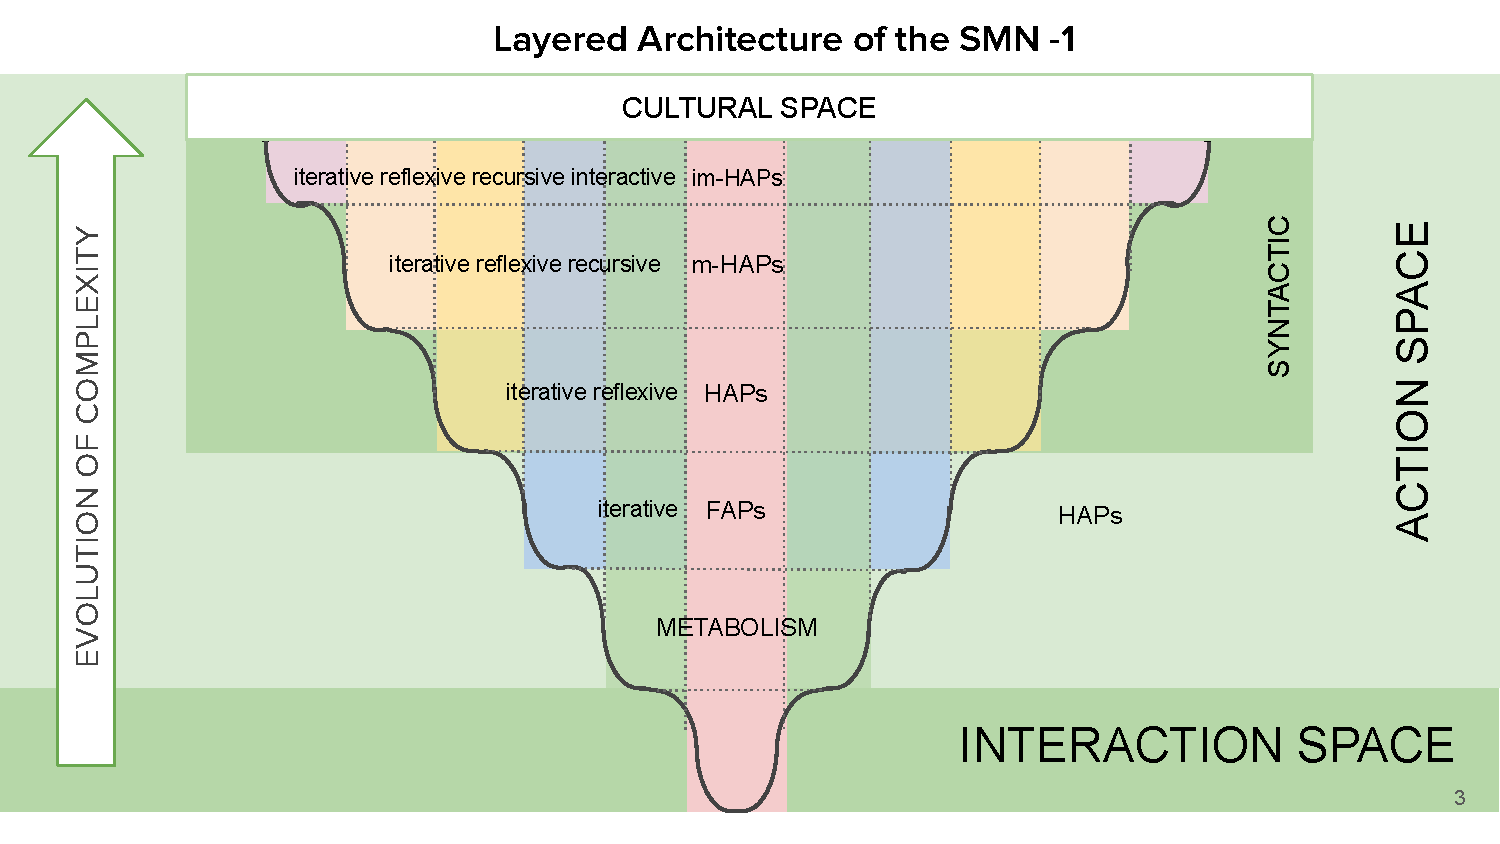
\includegraphics[width=\textwidth]{graphics/SideViewLayers.pdf}
\caption{\textbf{A schematic representing layered architecture of SMN.}}
\label{side_view_lSMN}
\end{figure}

\begin{figure}[ht] 
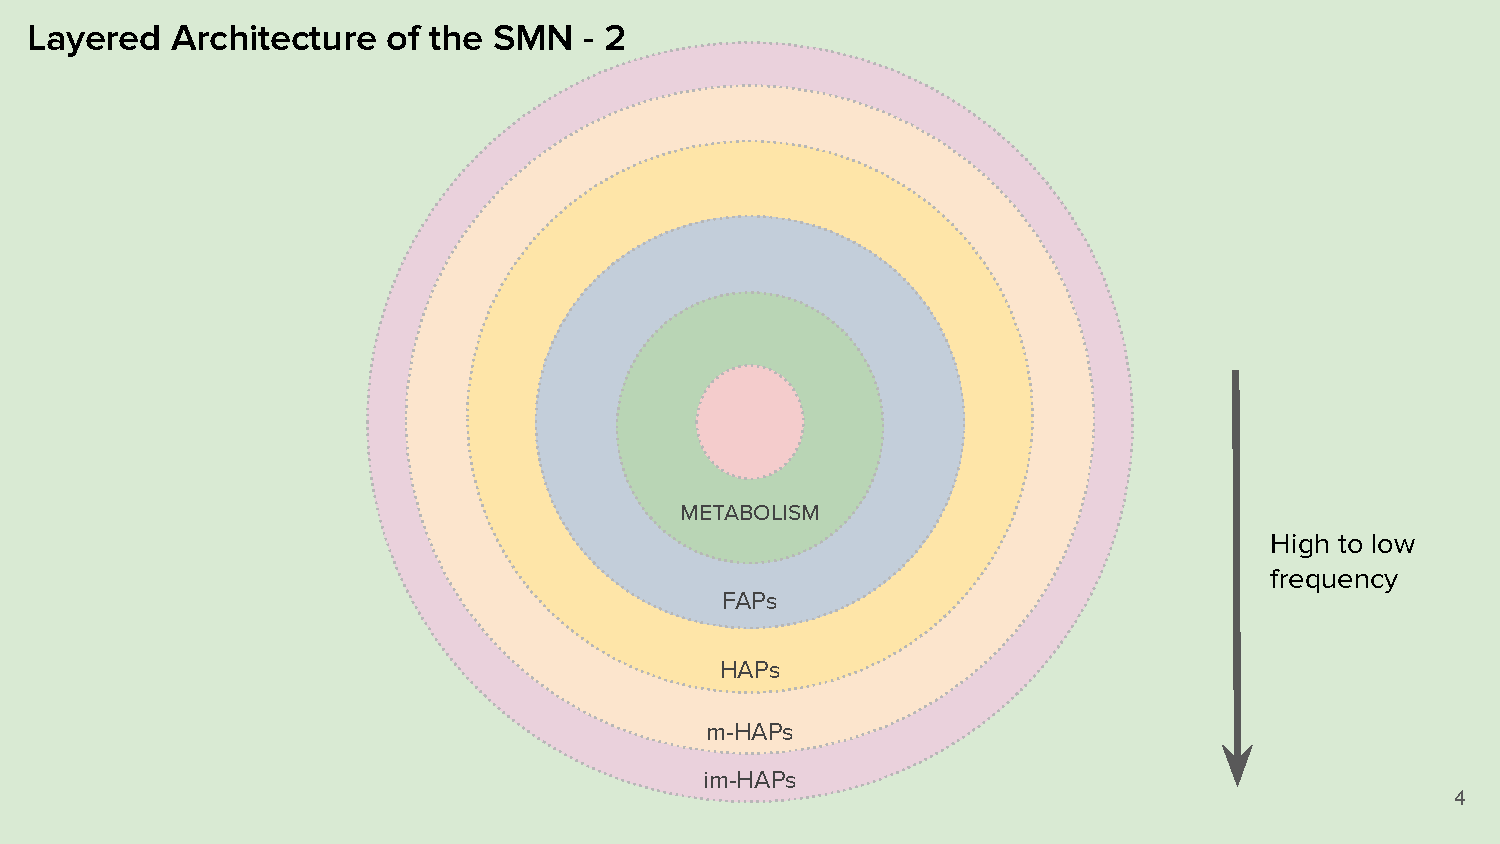
\includegraphics[width=\textwidth]{graphics/TopviewLayers.pdf}
\caption{\textbf{A schematic representing layered architecture from a top view.}}
\label{top_view_lSMN}
\end{figure}

\subsection{Learning and Memory Grounded in Affordability}
As repeatedly mentioned here, the units of cognition are action-patterns. Patterns are available both as constellations, i.e. as pictures or snapshots, as well as melodies, i.e. sequences or streams. The former are atemporal. The so-called atemporality of constellations is due to the stable relations over time. They are differentiated based on geometrical relations. The latter, like melodies, are differentiated on the basis of how the constellations vary over time. Relations are the discernibles which form patterns and the variations are the changes in relations. The core aspect of what we can discern are relations but not things per se. What stays as memory is nothing but stability of the pattern --- the relations in the constellations and melodies. Memory is not for action; action patterns \textit{are} memories. Therefore, this model suggests that memory is not a substance that can be stored but a reproducible pattern of relations. The apparent storage property of memory arises from the potential to reproduce.
This potential is a function of re-forming and de-forming the action patterns as FAPs and HAPs. This is a dynamic negotiation space and not something that can be described in terms of the binaries of innate and learnt. 

Affordability of holding an action pattern determines the ability of storing memory. Holding action patterns is expensive than holding the traces. The traces give us the apparent character of a storable memory. Though action patterns (both HAPs and FAPs) are transient, they can be reproduced. FAPs are easily reproduced and are triggered by the immediate environment, while reproducing HAPs requires additional triggers and practice. HAPs, as discussed earlier, can be saturated or unsaturated. As HAPs evolve into TAPs, the requirements of context and practice increase, while reducing the cost of storing. The spectrum from beats to TAPs is very broad. 

In the proposed model, we assume that the polarised and asymmetric architecture and the sensory motor network of the body is evolutionarily granted. Most of these aspects can be considered as evolutionarily learnt and genetically memorised, in a broader sense of the term ``memory''. However since the body plan and SMN aspects are crucial for cognitive development we can not ignore how dependent the phenomenon is on what is biologically granted. As we distinguish between interactions (molecular and cellular level) and actions (organ level), let us focus on the learning and memory related to the latter. 

The bridge between interactions and actions that have an important role in cognition is the layer of beats. Though variations in the beating patterns (heart beat and breathing pattern) are limited, these are triggered by both internal as well as external environment. Their potential in generating cognitive experiences can not be ignored. Often we might consider such experiences only within the bracket of emotions and feelings, in our framework they play very vital role in evaluatory interpretation of other actions, and this forms the site for grounding semantics. While we perform FAPs, HAPs and TAPs, we can not afford to cross the tolerance limits of variations possible by the spectrum of beats. There for this is a significant bridge between interactions and actions. The entire spectrum of learning and memory with respect to FAPs, HAPs, and TAPs are negotiable only within this affordability space. 

The body plan (through genetic memory) and the habitat (provided by the living context) determine the FAPs such as flipping of fins and tails, swallowing and undulation, walking, running, self-pruning etc. These FAPs form the habit-habitat coupling. Based on the affordances offered by the internal and external environments, a wide range of variations are possible in these action patterns. Though largely these are determined by genetic factors and the habitat, since these actions are performed by the SMN, they play the role of differentiating the difference in the habitat.Thus the extent of variations in action patterns increases by several folds once the FAPs layer enters the scene. The reproducibility of these variations in action patterns constitutes the memory in this layer. The motor action is almost inevitable in a live SMN, as evident in pre-natal FAPs. The initial trigger for FAPs is largely internal therefore genetic. Apart from the emotions and feelings, the FAPs are the action schemas, in Piagetian terms, using which the SMN explores the world. 

Over and above the genetically determined action schemas the affordances of the habitat trigger variations introducing gaps in the FAPs. As more bifurcations become possible enabling disengagement, the spectrum of variations possible within the FAPs enhances manifold which catapults the SMN into the layer HAPs. The flexible (dexterous) motor anatomy has the potential to transform (re-form) the network following the FTWT principle, which makes the SMN plastic. Without variations in the action patterns enabled by the motor anatomy (plasticity of the action zones), the new connections in the network are not possible (plasticity of network). We tend to propose the primacy of motor plasticity resulting into neuronal plasticity. This speculation is grounded in the evolutionary and embryological history (phylogeny and ontogeny), that all cells are capable of movement and communication with each other without neurons. However once neuronal connections are available in an organic structure, it is untenable to ascribe primacy of cognitive function to any one part of the SMN --- action-over-network or network-over-action. The newfound connections and newfound HAPs are indiscernible in a network architecture. Therefore it is untenable to say the memory is exclusively in the connecting units or in the motor units. Locating memory, is hence a untenable research project, except ascribing it to the entire network. However, as we move from HAPs to TAPs the locatable, storable, and retrievable nature of the traces of HAPs, representations, become possible. Insofar as the representations are available to the cognitive agent, they are manifested organically, as a whole, and therefore cannot be ascribed to any one part of the SMN. 

Memorisation or learning of HAPs is apparently contradictory in an interesting way. The emergence of a HAP is at the breaking of a pre-formed pattern. For HAPs require gaps, halts, breakages and new variations --- a creative force. Now, when we talk about memorisation and learning of HAPs, it is about reproducing the action pattern again and again. The orientation here is to sediment the pattern to FAPs to an extreme of establishing hard connections between the zones --- a conservative force. Once you learn a HAP very well, it ceases to be a HAP. An explanation for this could be that the FAPs are the attractors ---  the conserving and reproducing tendency --- of multiple zones of SMN as dynamical systems. It is therefore a matter of habit for a biological system, to repeat almost all happenstances. It is a default self-reproducing embodied force, as vindicated by autopoetic model of life, a kind of inertia in action. 

The biological order maintains a landscape of the SMN, where the topos of the landscape is determined by the body plan (polarised or not, symmetrical or not). The dynamical nature of the FAPs generate the attractors in the landscape. The available articulatory freedom, provided by the multiplicity of the action zones, gives rise to the soundscape, so to speak of the HAPs and TAPs. The soundscape is a transient state, and exists as long as the FAPs, HAPs and TAPs persist, which is the wakeful state. When the action zones are in a restful state, e.g. in a sleep, the soundscape is like a calm surface of a lake. This analogy with the active cognitive state as a soundscape and the biological body as the landscape can be mapped to the layered architecture of the SMN where the interactional space of the SMN forms the landscape, while the action space forms the soundscape.


\subsection{Editorial Checklist (to be removed before submission)}
\begin{itemize}
    \item Resolve all \todo{} items and promote selected \marginpar{} notes to footnotes if desired.
    \item Ensure cross-references (\cref{}) point to final section labels.
    \item Add citations for fluid dynamics, gravity priors, and thermodynamic arguments.
    \item Remove this checklist and the \texttt{Detailed Elaboration} subsection after merging.
\end{itemize}
